\cotefile{13}
\scanpage{11}
tout $s\in S$, $P_s$ le \unsure{torseur|torseurs} sur $G(\unsure{\mathbb{Q}|Q})$
\[
 P_s=\operatorname{Isom}_{\otimes}(\omega\inserted{\text{foncteur oubli}},\unsure{\Phi_s}F)
\]
Pour $s$ variable, les $P_s$ forment un revêtement principal \inserted{(à droite)} $P$ de $S$, de groupe $\Gamma=G(\mathbb{Q})$. On a tout ce qu'il fallait pour que le \unsure{$\otimes$} composé
\diagram{\begin{tikzcd}[ampersand replacement=\&,column sep=large]
 C=\operatorname{Rep}(G) \arrow[r,"F"] \& \operatorname{Hodge}(S) \arrow[r,"{V\mapsto V\times_S P}"] \& \operatorname{Hodge}(P)
\end{tikzcd}}
\deleted{\unsure{ait une struct|ait un struct}} \unsure{definisse|définisse} sur $P$ une $G$-\unsure{subordination}, d'où un morphisme
\[
 g:P\longrightarrow\unsure{\gamma|\mathcal{Y}}.
\]
\deleted{Ceci posé,} Ce dernier est compatible avec l'action de $\Gamma=G(\mathbb{Q})$\unsure{,|.} \inserted{(opérant sur $\gamma$ à \uline{droite}).} Et la catégorie des \deleted{\unsure{$\otimes$ foncteurs} $F$} $G$-subordinations $F$ sur $S$ compatibles avec le foncteur oubli est équivalente à celle des couples $(P,g)$, $P$ un rév. principal de $S$ de \unsure{gpe|groupe} $\Gamma$, $g:P\unsure{\relbar|\to}\gamma$ un $\Gamma$ morphisme.

Soit $\Gamma_0\subset\Gamma=G(\mathbb{Q})$ un \unsure{ss-gpe|ss-groupe} [de \unsure{préférence|préference|preférence}, commensurable à un $G(\mathbb{Z})$]. On appelle $G$-subordination $\Gamma_0$-\unsure{rigidifiée|rigidifiee} sur $S$ la donnée \unsure{d'une|d'un} rev. principal $P_0$ de $S$ de
% archive sheet number: 10
\scanpage{12}
\unsure{groupe|gpe} $\Gamma_0$, et d'un \unsure{$\Gamma_0$-hom|$P_0$-hom} de $P_0\longrightarrow\unsure{\gamma|\mathcal{Y}}$.

Si $\Gamma_0=\{e\}$, on trouve la notion de $G$-\unsure{subordination} \unsure{rigidifiée|rigidifiee}, si $\Gamma_0=G(\unsure{\mathbb{Q}|Q})$, la notion de $G$-subordination tout court. On peut expliciter la notion par la donnée d'un $F$\inserted{compatible avec $\omega$,}, et d'une \deleted{\unsure{sous}} $\Gamma_0$-rigidification de $F$ i.e. \unsure{un|une} sous-\unsure{fibre|fibré} $P_0$ de $P$, qui soit un \deleted{\unsure{sous}} $\Gamma_{0_S}$-torseur pour l'action naturelle de $\Gamma_{0_S}$\,\unsure{.....|....}

Pour cette structure, il y a un topos modulaire, qui n'est autre que \deleted{\unsure{$(\gamma,$a|$(\gamma,$}} $(\gamma,$ avec action de $\Gamma_0$ à droite). \unsure{$\forall$|Et} Le quotient $\gamma/\Gamma_0$ (avec sa structure d'espace analytique quand $\Gamma_0$ agit proprement comme groupe discret\unsure{]|)} \deleted{est} joue le \unsure{role|rôle} d'une \uline{variété} \uline{de \unsure{modul|moduli|module}} \uline{de niveau} $\Gamma_0$.
% archive sheet number: 11
\scanpage{21}
\begin{flushright}\begin{minipage}{.54\linewidth}
Descriptions transcendantes de motifs en car $0$ et de \unsure{catégories|catégorie} de motifs en car. $0$

\figure{\hspace{.16\linewidth}
\begin{tikzpicture}
 \draw[line width=.6pt,line cap=round] (0,0) .. controls (.55,.01) and (1.25,.03) .. (1.72,.14);
\end{tikzpicture}}

doubles réseaux \unsure{etc|et c}
\end{minipage}\end{flushright}

\vspace{1cm}
\figure{\hspace{.15\linewidth}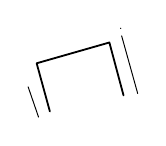
\begin{tikzpicture}[x=.012cm,y=-.012cm,line cap=round,line join=round]
 \draw[line width=.65pt] (24,97) -- (10,46) -- (87,24) -- (102,80);
 \draw[line width=.35pt] (1,71) -- (12,103);
 \draw[line width=.35pt] (100,17) -- (117,78);
 \fill (99,9) circle[radius=.7];
\end{tikzpicture}}

\vspace{3cm}
\figure{\hspace{-.17\linewidth}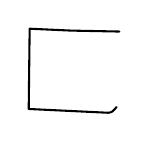
\begin{tikzpicture}[x=.012cm,y=-.012cm,line cap=round,line join=round]
 \draw[line width=.75pt] (98,4) -- (47,3) -- (3,1) -- (2,86) -- (86,90) .. controls (91,90) and (92,87) .. (95,84);
\end{tikzpicture}}
% archive sheet number: 20
\scanpage{23}
\deleted{Dans le cas général (motifs pas nécessairement constants) la connaissance des opérations $\Theta_X$ sur les $V_{\unsure{\mathbb{C}|C}}$ $(V\in\operatorname{Ob}\unsure{\mathcal{M}|M})$ implique-t-elle celle des \unsure{éléments} des structures $1^{\mathrm o}$ et $2^{\mathrm o}$, \deleted{ou dans quelle mesure du moins?}}
\margin{\deleted{\uuline{\unsure{oui}}} ??}

\margin{
\begin{tikzpicture}
\node[inner sep=1pt,align=left,text width=.93\marginparwidth] (rubrique) {Situation abstraite de la donnée d'une connexion \unsure{intégrable} \unsure{sur|un} foncteur fibre.};
\draw (rubrique.north west) -- (rubrique.south west) -- (rubrique.south east);
\end{tikzpicture}}

\begin{center}\rule[.2ex]{2cm}{.4pt}\end{center}

Considérons une $\otimes$-catégorie $\mathcal{M}$ sur corps $k_0$, soit $K$ une extension de $k_0$. On suppose donné un foncteur fibre à valeurs \unsure{en|ds} $k_0$, \unsure{donc|dans} $\mathcal{M}$. avec ce foncteur fibre est donné par $G$ sur $k_0$, ($\mathcal{M}$ s'identifie \unsure{avec|aux} \unsure{``$G$-$k_0$-modules\ldots|$G$-$k_0$-modules\ldots} On veut déterminer les façons de mettre\unsure{,} sur chaque $V\otimes_{k_0}K$ une connexion intégrable \inserted{\unsure{rel|rel.} à $K/k_0$}, \uline{fonctorielle} en $V$, \inserted{et ``\unsure{compatible|compatibles} avec $\otimes$''.}

Or il y en a déjà une $\Theta_0$, \unsure{déduit|déduite} des \unsure{$k$-|$k_0$-}structures dont on \deleted{\unsure{suppose}} dispose déjà sur chaque $V\otimes_{k_0}K$. Une autre connexion \deleted{\unsure{intégrable}} \inserted{sur $V$} sera donc de la forme
\[
 \Theta_X^V={\Theta_0}_X^V+\omega^V(X)^{\deleted{\unsure{V|x}}}
\]
\unsure{où|ou}
\[
 \omega^V\deleted{\unsure{(X)|\in}}:\operatorname{Dér}_{\unsure{k|k_0}}(K/k_0)\longrightarrow
 \operatorname{End}_K(V_K\unsure{)}\,\text{est \uline{$K$-linéaire}}
\]
\[
 \Theta_X^V(\unsure{\varphi|\phi})={\Theta_0}_X^V(\varphi)+\omega^V(X)(\varphi)
\]
Si on veut choisir les $\Theta_X^V$ pour tt $V$, de façon compatible avec multiplication, on trouve que \deleted{$\unsure{\omega^V|\omega}\unsure{\Theta_X|(X)}$} $\omega^V(X)$, pour $V$ variable, est une ``dérivation'' du foncteur fibre \deleted{\unsure{donné}}\inserted{$F_K$}, donc défini par un élément de \deleted{Lie} $\unsure{\mathfrak{g}|\mathcal{G}}_K$, où $\mathfrak{g}=\operatorname{Lie}G$. Soit $\omega(X)\in\mathfrak{g}_K$ cet élément\unsure{.|,}
% archive sheet number: 22
\scanpage{24}
on trouve donc $X\unsure{\relbar|\mapsto}\omega(X):\operatorname{Dér}(K/k_0)\unsure{\relbar|\to}\unsure{\mathfrak{g}|\mathcal{G}}_{\unsure{k|K}}$, application $K$-linéaire :
\[
 \omega:\operatorname{Der}(K/k_0)\longrightarrow\mathfrak{g}_K
\]
\unsure{Si} on veut avoir des connexions \uline{intégrables}, il faut écrire de plus la condition d'intégrabilité
\[
 \overbrace{{\Theta_0}_X\omega(Y)-{\Theta_0}_Y\omega(X)}^{\inserted{\mathrm{d}\omega(X\wedge Y)}}
 \deleted{\unsure{+[\omega(X),\omega(Y)]|-[\omega(X),\omega(Y)]}}
 =\omega([X,Y])-[\omega(X),\omega(Y)]
\]
où \deleted{\unsure{$\Theta_0$|On}} $X,Y\in\operatorname{Dér}(K/k_0)$ et ${\Theta_0}_X$, \inserted{${\Theta_0}_Y$} opèrent sur $\mathfrak{g}_K=\mathfrak{g}\otimes_{k_0}K$ via les op. sur $K$.... .

Le plus souvent, on aura en fait
\[
 \omega\in\Omega^1_{K/k_0}\otimes_K\mathfrak{g}_k
 \quad(=\Omega^1_{K/k_0}\otimes_{k_0}\mathfrak{g}_{\deleted{\unsure{K|k}}})
\]
de sorte que $\omega$ provient déjà d'un élément
\[
 \omega_{\deleted{\unsure{K}}k}\in\Omega^1_{k/k_0}\otimes_k\mathfrak{g}_k
\]
où $k$ est une ext. de type fini de $k_0$ (N.B. si $k$ est fixé, $\omega_k$ est uniquement déterminé, si on est en \uline{car. $0$}). La donnée de $\omega_k$ \unsure{revient|équivaut|révient} aussi à la donnée d'un hom $k_0$-linéaire
\[
 \Omega=\mathfrak{g}^{\unsure{\vee|V}}\longrightarrow\Omega^1_{k/k_0}\quad(\longrightarrow\Omega^1_{K/k_0})
\]

Nous allons examiner à quelles conditions, \deleted{\unsure{tout hom|tous les hom}} pour $V,W\in\operatorname{Ob}\unsure{\mathcal{M}|M}$ donnés, \deleted{\unsure{les}} hom \inserted{\uline{de $k_0$-\unsure{vectoriels|vecteurs}}} $u:V_{\deleted{\unsure{K}}}\longrightarrow W_{\deleted{\unsure{K}}}$ \deleted{qui} \inserted{tels que $u_K:V_K\unsure{\relbar|\to}W_K$} commutent \unsure{avec|aux} $\Theta_{\unsure{x|X}}$ $(X\in\operatorname{Dér}(K/k_0))$ \deleted{\unsure{soit|sont}} commutent à $G$, en supposant $G$ connexe ($k_0$ de car. $0$). Il suffit
% archive sheet number: 23
\scanpage{25}
d'écrire que $u_K$ commute à $\unsure{\mathfrak{g}|\mathcal{G}}_K$, or par hyp. il commute aux $\omega(X)\in\mathfrak{g}_K$ $(X\in\operatorname{Dér}(\unsure{H|\Pi|K}/k_0)\unsure{]|)}$, Soit $\unsure{\mathfrak{u}|\mathfrak{a}|U}\subset\mathfrak{g}$ le plus petit \unsure{sous-espace} vectoriel de $\mathfrak{g}$ tel que $\mathfrak{u}_K$ contienne les $\omega(X)$. Alors il est clair (alg. linéaire) que \deleted{$\unsure{\mathfrak{u}|u_K}$} $u$ commute à $\mathfrak{u}$, donc il suffit que $\mathfrak{u}=\mathfrak{g}$ pour pouvoir conclure (N.B. Il suffirait que l'\unsure{algèbre|Algèbre|algébre} de Lie engendrée par $\mathfrak{u}$ dans $\mathfrak{g}$ soit $\mathfrak{g}$, mais en fait on se convainc facilement que $\mathfrak{u}$ est déjà une $\unsure{k|K}$-algèbre de \unsure{Lie|bie}....). On peut $\unsure{\overline{\mathrm m}|\overline{\mathrm{m\!m}}}$ remplacer $\mathfrak{u}$ par l'algèbre de Lie \unsure{algébrique} qu'elle engendre
% archive sheet number: 24
\scanpage{27}
\begingroup\makeatletter\tagsleft@true\makeatother
\margin{\begin{tikzpicture}
\node[inner sep=1pt,align=left,text width=.93\marginparwidth] (titre) {structure filtrée sur DR et comparaison avec Betti, Hdg...};
\draw (titre.north west) -- (titre.south west) -- (titre.south east);
\end{tikzpicture}}

Soit $k\unsure{\mathrel{\tikz[x=.58em,y=.58em,baseline=0pt,line cap=round]{\draw (.87,.44) .. controls (.60,.70) and (-.03,.34) .. (.04,.17) .. controls (.12,.04) and (.78,.09) .. (1.20,.02); \draw (1.23,.14) -- (1.14,.80) .. controls (1.15,.96) and (.92,.79) .. (.99,1.00) .. controls (1.01,1.08) and (1.05,1.12) .. (1.09,1.13);}}|\subset^{\iota}|\subset}\mathbb{C}$, considérons une \unsure{catégorie.|catégor.} de motifs \inserted{sur $k$,} de type fini \deleted{\unsure{soit}}, soit $\mathcal{M}$. Il y a deux foncteurs fibres naturels,
\[
T_{\mathrm{DR}}:\mathcal{M}\unsure{\relbar|\longrightarrow}\operatorname{Mod}f(k)\tag*{(1)}
\]
\diagram{\begin{minipage}{\linewidth}
\[
\begin{tikzcd}[ampersand replacement=\&,column sep=1.2em]
T_{B\unsure{\mathrm{dg}|\mathrm{Hdg}|\mathrm{tg}}}:\mathcal{M}\arrow[r]\&
\deleted{\operatorname{Mod}f(\unsure{\mathbb Q|Q})}\ \mathrm{Str.}\ \mathrm{Hodge}\arrow[r]\&
\operatorname{Mod}f(\mathbb Q),
\end{tikzcd}\tag*{(2)}
\]
\end{minipage}}
le deuxième dépendant de l'imm. $k\subset\mathbb{C}$. Le premier a une structure de filtration. De plus, on a un isom canonique
\[
\unsure{\varphi|\phi}:T_B\otimes_{\mathbb Q}\mathbb C\xrightarrow{\sim}T_{\mathrm{DR}}\otimes_k\mathbb C\tag*{(3)}
\]
\inserted{compatible aux filtrations des 2 \unsure{mbres|mbrs}}

Soit $G$ gpe des Aut. de $T_B$. Comparant $T_{\mathrm{DR}}$ et $T_{\unsure{B|D}}\otimes_{\mathbb Q}k$, on trouve un torseur à droite
\[
P=\unsure{\underline{\operatorname{Isom}}|\underrightarrow{\operatorname{Isom}}}_{\otimes}(T_B\otimes_{\mathbb Q}k,T_{\mathrm{DR}})\tag*{(4)}
\]
sous $G_k$, qui permet de récupérer le foncteur $T_{\mathrm{DR}}$ comme
\[
T_{\mathrm{DR}}=\deleted{T_B\otimes}\ P\overset{G_k}{\times}(T_B\otimes_{\mathbb Q}k).\tag*{(5)}
\]
De plus, \deleted{\unsure{on a un isom.}} l'isom (3) définit un élément canonique
\[
\varphi\in P(\mathbb C)
\]
\margin{\begin{tikzpicture}
\node[inner sep=1pt,align=left,text width=.91\marginparwidth] (note) {La connaissance de $G,P,\varphi$ permet de récupérer ess. $\mathcal M$ avec (1) (2) et (3)};
\draw ([xshift=1pt]note.north west) -- ([xshift=-3pt]note.south west);
\end{tikzpicture}}% slanted

Pour récupérer la structure filtrée sur $T_{\mathrm{DR}}$, \deleted{et} donc la structure de Hodge sur $T_B$ i.e la bigraduation sur $T_B\otimes_{\mathbb Q}\unsure{C|\mathbb C}$, il convient d'introduire
\[
T_{\mathrm{Hdg}}\unsure{\in|\mathord{:}}\mathcal M\longrightarrow\operatorname{Mod}\deleted{\unsure{\mathrm{Bi}|\mathrm B}}\mathrm{grad}\,f(k),\qquad T_{\mathrm{Hdg}}=\operatorname{gr}^{*}T_{\mathrm{DR}}.\tag*{(6)}
\]
\inserted{Soit} \deleted{et les deux \unsure{groupes|grpes} de} \deleted{\unsure{Lie}}
\[
\deleted{\unsure{H|K}}\ G'_k=P\overset{G_k}{\times}G_k=\operatorname{ad}(P)\simeq\underline{\operatorname{Aut}}_{\otimes}(T_{\mathrm{DR}})\tag*{(7)}
\]
\deleted{\unsure{Ainsi|Alors}} et
\[
\begin{aligned}
H'\subset G'_k\qquad &\text{\unsure{ss grpe|ss groupe} des $\otimes$-Aut de $T_{\mathrm{DR}}$ respectant}\\
&\text{la filtration et qui induisent l'}\\
&\text{identité sur le gradué associé.}
\end{aligned}\tag*{(8)}
\]
\endgroup
% archive sheet number: 26
\scanpage{28}
\begingroup\makeatletter\tagsleft@true\makeatother
C'est un groupe unipotent, et on peut introduire
\[
Q=\underline{\operatorname{Isom}}_{\substack{\otimes,\,\text{ind. l'ident.}\\\text{sur }\operatorname{gr}^{*}}}(T_{\mathrm{DR}},T_{\mathrm{Hdg}}),\tag*{(9)}
\]
de sorte que $Q$ est un torseur à droite sous $H'$. Posons

\reversemarginpar
\margin{\figure{\begin{tikzpicture}[x=0.42cm,y=0.42cm]
\draw[->] (0.4,-3.3) .. controls (-0.55,-1.5) and (-0.05,-0.6) .. (0.55,-0.45) .. controls (1.3,-0.25) and (2.1,-0.13) .. (2.9,0.25);
\draw (1.5,-3.08) .. controls (1.12,-3.32) and (0.51,-3.05) .. (0.45,-3.3);
\draw (0.52,-3.34) .. controls (0.38,-3.92) and (0.67,-4.08) .. (1.12,-4.04);
\end{tikzpicture}}}
\normalmarginpar
\[
\begin{aligned}
\deleted{\unsure{G''|G'}}\ H''=Q\overset{H'}{\times}H=\operatorname{ad}(H')&\simeq\deleted{\unsure{\operatorname{Aut}}}\ \text{ss-gpe de}\\
&H''=\underline{\operatorname{Aut}}_{\unsure{\ominus|\otimes}}(T_{\mathrm{Hdg}})\ \text{respectant}\\
&\text{la filtration associée}\\
&\text{à la bigraduation,}\\
&\text{et induisant l'identité}\\
&\text{sur gradué}\\
&\text{associé --}
\end{aligned}\tag*{(1\deleted{\unsure{0|1}}\unsure{1|0})}
\]
\[
G''=Q\overset{H'}{\times}G'=\underline{\operatorname{Aut}}_{\ominus}(T_{\mathrm{Hdg}}).\tag*{(10)}
\]
Alors la bigraduation de $T_{\mathrm{Hdg}}$ définit
\[
i_1,i_2:\unsure{G_{m_k}|G_{m\,k}}\unsure{\relbar|\longrightarrow}G'\tag*{(12)}
\]
satisfaisant
\[
\unsure{\varepsilon|\epsilon}i_1(\lambda)=\varepsilon i_2(\lambda)=\lambda,\qquad \unsure{i_1|i'_1}(\lambda)i_2(\lambda)=\unsure{i|i'}(\lambda).\tag*{(13)}
\]

Ainsi, on obtient les données suivantes

\begin{enumerate}[label=\alph*)]
\item Groupe algébrique $G$ sur $\unsure{\mathbb Q|Q}$, avec \diagram{\begin{tikzcd}[ampersand replacement=\&,column sep=small]G_m\arrow[r,"i",no head]\& G\arrow[r,"\varepsilon",no head]\& G_m\ \ldots\end{tikzcd}}
\item Groupe algébrique $G''$ sur $k$, avec \diagram{\begin{tikzcd}[ampersand replacement=\&,column sep=small]G_m\arrow[r,"i''",no head]\& G''\arrow[r,"\varepsilon''",no head]\& G_m\ \ldots\end{tikzcd}}
\item hom $i_1,i_2$ (12) satisfaisant les conditions (13)
\item Torseur \inserted{à g.} $Q$ sous le groupe \inserted{unipotent} $H''$ \inserted{$\subset G''$} défini par $(G'',\unsure{i_1|i_+})$\deleted{\unsure{le|de}}

On considère alors $\deleted{\unsure{Q\overset{H''}{\times}G''=|Q\overset{H'}{\times}G'=}}$
\[
\left\{\begin{aligned}
H'&=H''\overset{H''}{\times}Q=\operatorname{ad}_{H''}(Q)\\
\makebox[0pt][r]{\smash{\raisebox{-.8ex}{\parbox[c]{1.05em}{\figure{\tikz[x=.6em,y=.8em]{\draw[->] (.55,1.4) .. controls (-.30,1.13) and (-.27,.05) .. (.72,-.08);}}}}}\hspace{.25em}}G''&\overset{H''}{\times}Q=\unsure{P|Q}\qquad\text{(tors. à g. sous $G''$)}\\
G'&=G''\overset{G''}{\times}Q\unsure{\mathord{:}|=}\operatorname{ad}_{G''}(Q)
\end{aligned}\right.
\]
[NB, $Q$ est trivial, donc $G'\simeq G''$ (pas canoniquement], puis
\item Torseur à g. $\unsure{P|\mathord{?}}$ sous $G'$, \deleted{avec un \unsure{isomorphisme|homomorphisme} de \unsure{$G_m\overset{G'}{\times}P$|$G'\overset{G'}{\times}P$}.}
\deleted{On considère alors $G$}
\item Un isom $G\otimes_{\mathbb Q}k\simeq G'\overset{\unsure{G'|B'}}{\times}\unsure{P^{*}|P}=\operatorname{ad}_{G'}(P)$ \margin{compatible avec les structures $i,\varepsilon$}
\item[] \deleted{\unsure{g) un|g) Un}} g) Un élément \deleted{\unsure{de|en}} $\unsure{\varphi|\phi}\in P(\mathbb C]$, \deleted{\illegible{1}}
\end{enumerate}
\endgroup
% archive sheet number: 27
